\chapter{SAX-VSM: A Novel Technique For Interpretable Time Series Classification}\label{chapter_sax_vsm}

\textit{In this chapter I show a novel algorithm for interpretable time-series classification based on
characteristic patterns discovery. }

\section{Background}
Time series classification is an increasingly popular area of research, providing 
solutions to a wide range of fields, including data mining, 
image and motion recognition, environmental sciences, health care, and chemometrics. 
Within the last decade, many time series representations, similarity measures, 
and classification algorithms were proposed following the rapid
progress in data collection and storage technologies \cite{citeulike:10358271}. 
NNevertheless, to date, the best overall performing classifier in the field is
the nearest-neighbor algorithm (1NN), that can be easily tuned for a 
particular problem by choosing either a distance measure, 
an approximation technique, or smoothing \cite{citeulike:11796594}. 
The 1NN classifier is simple, accurate and robust, depends on a very few parameters 
and requires no training \cite{citeulike:10358271, citeulike:532340, citeulike:11796594, citeulike:12563424}. 
However, the 1NN technique has a number of significant disadvantages, 
where the major shortcoming is the inability to offer any insight into the classification results.
Another limitation is its need for a significantly large training set 
representing a within-class variance in order to achieve desired accuracy. 
Finally, while having trivial initialization, 1NN classification is computationally expensive. 
Thus, the demand for an efficient and interpretable classification technique 
capable of processing of large data volumes remains.

In this thesis, I propose an alternative to 1NN algorithm that addresses 
aforementioned limitations. Specifically, it provides a superior interpretability, 
learns efficiently from a small training set, and has a low classification 
computational complexity. As I shall show in the following chapters, these algorithm's
properties, make it the best choice for the problem in hands.

\section{Prior and related work} \label{prior}
Almost all of the existing techniques for time series classification can be divided 
in two major categories \cite{citeulike:10249370}. 
The first category includes techniques based on shape-based similarity metrics 
where distance is measured directly between time series points. 
Classical examples from this category is 1NN classifier 
built upon Euclidean distance \cite{citeulike:4214336} or DTW \cite{citeulike:3496861}. 
The second category consists of classification techniques based on 
structural similarity metrics, which employ a high-level representations 
of time series based on their global or local features. 
Examples from this category include classifiers based on 
time series representation obtained with Discrete Fourier Transform \cite{citeulike:5094223}
or Bag-of-Patterns \cite{citeulike:10525778}. 
The development of these distinct categories can be explained by 
the difference in their performance: 
while shape-based similarity methods are virtually unbeatable on short 
pre-processed time series \cite{citeulike:532340}, 
they usually fail on long and noisy data sets 
where structure-based solutions demonstrate a superior performance \cite{citeulike:12563380}. 
In addition, structure-based methods usually memory and runtime-effective, 
thus, they often implemented in industrial settings. 

Additionally, in the context of my work, it is worth to note, that classification 
techniques from both categories can be also attributed as exact or approximate.
While former are based on exact metrics, and typically are brute force 
algorithms which guarantee results through an exhaustive search, 
the latter are usually built upon an approximate representation of 
time series, or upon an approximate similarity metric, and do not guarantee 
global correctness. Nevertheless, while allowing a potentially higher error rate,
approximate techniques effectively reduce the search space, thus dealing with 
large unprocessed data much more efficiently.


As possible alternatives to these two categories, two relevant to my approach techniques, 
were recently proposed. The first technique is the time series shapelets algorithm,
that was introduced in \cite{citeulike:7344347} and is featuring a superior interpretability 
and a compactness of delivered solution. 
A Shapelet is a short time series ``snippet'' that is a representative of class
membership and is used for a decision tree construction facilitating class 
identification and interpretability. In order to find a branching shapelet, 
the algorithm exhaustively searches for a best discriminatory shapelet on data split via 
an information gain measure. The algorithm's classification is built upon the similarity 
measure between a branching shapelet and a full time series, defined as a distance 
between the shapelet and a closest subsequence in the series when measured by the 
normalized Euclidean distance.  
This exact technique, potentially, combines the superior precision of 
exact shape-based similarity methods, and the high-throughput 
classification capacity of feature-based approximate techniques. 
However, while demonstrating a superior interpretability, robustness, 
and similar to 1NN algorithm performance, shapelets-based technique is 
computationally expensive, $O(n^{2}m^{3})$, where $n$ is a number of 
objects and $m$ is the length of a longest time series, making 
its adoption for many-class classification problems difficult \cite{citeulike:11345338}. 
While the faster solution was recently proposed ($O(nm^{2})$), it is an 
approximate solution that is based on indexing \cite{citeulike:12563493}.

The second technique with interpretable results is 1NN classifier built upon the 
Bag-Of-Patterns (BOP) representation of time series \cite{citeulike:10525778},
which is equated to an Information Retrieval (IR) ``bag of words" concept 
and is obtained by extraction, transformation with Symbolic Aggregate 
approXimation (SAX) \cite{sax}, and counting the frequencies
of short overlapping subsequences (patterns) along the time series.
By applying this procedure to a training set, the algorithm converts the data into 
the vector space, where the original time series are represented by a 
pattern (SAX word) occurrence frequency vector. 
These vectors are classified with 1NN classifier built with Euclidean distance 
or Cosine similarity applied to raw frequencies or their \textit{tf$\ast$idf} weighting. 
It was shown that BOP has several advantages: its complexity is linear 
($O(nm)$), it is rotation-invariant and considers local and global structures 
simultaneously, and it provides an insight into patterns distribution through 
frequency histograms.
The authors concluded, that the best classification accuracy of BOP-represented 
time series is achieved by using 1NN classifier based on Euclidean distance.

The proposed algorithm has similarities with aforementioned techniques. 
Similarly to shapelet-based approach, it finds time series subsequences
which are characteristic representatives of a whole class, thus enabling
superior interpretability.
However, instead of recursive search for discriminating shapelets, 
the algorithm ranks by “importance” all potential candidate subsequences 
\textit{at once} with a \textit{linear computational complexity} of $O(nm)$.
To achieve this, similarly to BOP, \mbox{SAX-VSM} converts all of the 
training time series into the vector space and computes tf$\ast$idf ranking.
But instead of building of $n$ bags (for each of the training time series), 
the algorithm builds a \textit{single bag of words for each of classes}, 
that effectively provides a compact solution of $N$ weight vectors 
($N$ is the number of classes, $N<<n$), and a fast classification time of $O(m)$.

As I shall show, these distinct features: the generalization of the class' 
patterns with a single bag and tf$\ast$idf ranking, allow SAX-VSM 
to achieve high accuracy, and tolerate noise in data.

\section{Background} \label{background}
SAX-VSM is based on two well-known techniques. The first technique is 
Symbolic Aggregate approXimation \cite{sax}, which is a high-level symbolic  representation 
of time series data. The second technique is a well known in Information Retrieval (IR) 
Vector Space Model \cite{citeulike:300428}. By utilizing a sliding window subsequence extraction and SAX, 
our algorithm transforms labeled time series into collections of SAX words (terms). 
At the following step, it utilizes \textit{tf$\ast$idf} terms weighting for a classifier construction. 
The SAX-VSM classification relies on cosine similarity metric.

SAX, however, requires two parameters to be provided as an input and 
no efficient solution for their selection exists to the best of my knowledge. 
I address this issue by using an optimization scheme based on the dividing 
rectangles (DIRECT) algorithm that does not require any input \cite{citeulike:12563460}. 
DIRECT is a derivative-free optimization process that possesses local and global optimization properties. 
It converges relatively quickly and yields a deterministic, optimized solution.

\subsection{Symbolic Aggregate approXimation (SAX)}
Symbolic representation of time series, once introduced \cite{citeulike:2821475}, has attracted much attention by
enabling an application of numerous string-processing algorithms, bioinformatics, and text mining 
tools to temporal data. The method provides a significant reduction of the time series 
dimensionality and a low-bounding to Euclidean distance metric, which guarantees no false 
dismissal \cite{citeulike:3175749}.
These properties are often leveraged by other techniques, which embed SAX representation 
in their algorithms for indexing and approximation. For example, adoption of SAX indexing 
allowed significant shapelets discovery speed improvement in Fast-Shapelets \cite{citeulike:12563493}
(but made the algorithm approximate).

%Given a time-series $T$ of a length $n$, SAX produces its symbolic approximation $\hat{S}$ of 
%a length $w$ where letters are taken from an alphabet $\alpha$. 
%Along with $T$, two parameters must be specified as the input: an alphabet size $\alpha$ and 
%a size of the word to produce $w$. Algorithm works as follows. 

%At first, since SAX rests on the assumption that normalized time series tend to have Gaussian 
%distribution \cite{larsen_marx}, the time-series $T$ is normalized to unit of standard deviation
%\cite{goldin_kanellakis}. 
%At the second step, the dimensionality of the normalized time series is reduced to $w$ by 
%obtaining a Piecewise Aggregate Approximation (PAA) of $T$. 
%Specifically, this approximation is obtained by dividing the time series $T$ into $w$ 
%equal-sized segments and computing the mean values for points within each segment. 
%The aggregated sequence of these mean values forms PAA approximation of $T$ of length $w$.
%Finally, each of PAA coefficients is converted into a letter of the alphabet $\alpha$ by the use 
%of lookup tables. These tables are built by defining a set of breakpoints that divide the 
%distribution space into $\alpha$ equiprobable regions \cite{sax}.
Configured by two parameters - a desired word size $w$ and an alphabet size $A$,
SAX produces a symbolic approximation of a time-series $T$ of a length $n$ by compressing 
it into a string of the length $w$ (usually $w<<n$), whose letters are taken from 
the alphabet $\alpha$ ($|\alpha|=A$). 
At the first step of the algorithm, $T$ is z-normalized (to unit of standard deviation)
\cite{citeulike:3815880}. 
At the second step, a dimensionality of the normalized time series is reduced from $n$ to $w$ by
obtaining its Piecewise Aggregate Approximation (PAA) \cite{citeulike:4406444}; for this, the normalized time
series is
divided into $w$ equal-sized segments and mean values for points within each segment are computed.
The aggregated sequence of these mean values forms PAA approximation of $T$. Finally, each of $w$
PAA coefficients is converted into a letter of an alphabet $\alpha$ by the use of the lookup table.
This table is pre-built by defining a set of breakpoints that divide the normalized time series
distribution 
space into $\alpha$ equiprobable regions. The design of these tables rests on the assumption 
that normalized series tend to have Gaussian distribution \cite{citeulike:10141990}.

\subsection{Bag of words representation of time series} \label{bow_representation}
Following its introduction, SAX was shown to be an efficient tool for solving problems 
of finding motifs and discords in time series \cite{citeulike:3977965, citeulike:3175749}. 
The authors employed a sliding window-based subsequence extraction technique 
and augmented data structures (hash table in \cite{citeulike:3977965} and trie in \cite{citeulike:3175749}) 
in order to build SAX words ``vocabularies''. Further, by analyzing words frequencies 
and locations, they were able to capture frequent and rare SAX words representing 
motifs and discords subsequences. Later, the same technique based on the combination 
of sliding window and SAX was used in the numerous works, most notably in time series 
classification using bag of patterns \cite{citeulike:10525778}. 

We also use this sliding window technique to convert a time series $T$ of a length $n$ into 
the set of $m$ SAX words, where $m=(n-l_{s})+1$ and $l_{s}$ is the sliding window length. 
By sliding a window of length $l_{s}$ across time series $T$, extracting subsequences, 
converting them to SAX words, and placing these words into an unordered collection, 
we obtain the \textit{bag of words} representation of the original time series $T$.

\subsection{Vector Space Model (VSM) adaptation}
We use Vector space model exactly as it is known in information retrieval (IR) \cite{citeulike:300428}. 
Similarly to IR, we define and use terms \textit{document}, \textit{bag of words}, 
\textit{corpus}, and \textit{sparse matrix} in our workflow. 
Note however, that we use terms \textit{bag of words} and \textit{document} 
for abbreviation of an unordered collection of SAX words interchangeably, while 
in IR these usually bear different meaning, where a \textit{document} usually 
presumes certain words ordering (semantics). 
Although, similar definitions, such as \textit{bag of features} or 
\textit{bag of patterns}, were previously proposed for techniques built upon 
SAX \cite{citeulike:10525778}, we use \textit{bag of words} since it reflects our 
workflow precisely. The term \textit{corpus} is used for a structured collection 
of bags of words. 

Given a training set, SAX-VSM builds bags of SAX-generated words representing 
each of the training classes and assembles them into a corpus. 
This corpus, by its construction, is a sparse \textit{term frequency matrix}. 
Rows of this matrix correspond to the set of all SAX words found in 
\textit{all classes}, while each column of the matrix denotes a class of the 
training set. Each element of this matrix is an observed frequency of a word
in a class. 
Many elements of this matrix are zeros - because words extracted from one class 
are often not found in others (Figure \ref{fig:venn}). 
By its design, this sparse 
term frequency matrix is a dictionary of all SAX words extracted from all time 
series of a training set, which accounts for frequencies of each word in each of 
the training classes.

Following to the common in IR workflow, we employ the \textit{tf$\ast$idf} weighting 
scheme for each element of this matrix in order to transform a frequency value into
the weight coefficient. 
The \textit{tf$\ast$idf} weight for a term is defined as a 
product of two factors: term frequency (\textit{tf}) and inverse document 
frequency (\textit{idf}). 
For the first factor, we use logarithmically scaled term frequency \cite{citeulike:4469058}:
\begin{equation}
 \mbox{tf}_{t, d} =  \begin{cases} \log(1 + \mbox{f}_{t,d}), &\mbox{if f}_{t,d}>0  \\
0, & \mbox{otherwise} \end{cases}
\end{equation} 
where $t$ is the term, $d$ is a bag of words (a \textbf{d}ocument), and $\mbox{f}_{t,d}$ 
is a frequency of the term in a bag.

The inverse document frequency we compute as usual:
\begin{equation}
 \mbox{idf}_{t, D} =  \log_{10}\frac{|D|}{|d \in D : t \in d|} = \log_{10}\frac{N}{\mbox{df}_{t}}
 \label{formula:idf}
\end{equation} 
where $N$ is the cardinality of corpus $D$ (the total number of classes) and the 
denominator $\mbox{df}_{t}$ is a number of documents where the term $t$ appears.

Then, $\textit{tf$\ast$idf}$ value for a term $t$ in the document $d$ of a corpus $D$ is defined as 
\begin{equation}
 \mbox{tf * idf}(t, d, D) =  \mbox{tf}_{t, d} \times \mbox{idf}_{t, D} = \log(1 + \mbox{f}_{t,d})
\times \log_{10}\frac{N}{\mbox{df}_{t}}
 \label{formula:tfidf}
\end{equation} 
for the all cases where $\mbox{f}_{t,d}>0$ and $\mbox{df}_{t}>0$, or zero otherwise.
Once all terms of a corpus are weighted, the columns of a sparse matrix are used 
as \textit{class term weights vectors} that facilitate the classification using cosine similarity. 

\enlargethispage{0.5cm} 
Cosine similarity measure between two vectors is based on their inner product. 
For two vectors $\mathbf{a}$ and $\mathbf{b}$ that is:
\begin{equation}
%\mbox{similarity}(\boldsymbol{a},\boldsymbol{b}) = cos(\theta) = \frac{ \sum\limits^{n}_{i=1} a_{i}
%\times b_{i} }{
%\sqrt{\sum\limits^{n}_{i=1} a_{i}} \times \sqrt{\sum\limits^{n}_{i=1} b_{i}} }
\mbox{similarity}(\mathbf{a},\mathbf{b}) = cos(\theta) = \frac{ 
\mathbf{a} \cdot \mathbf{b} } {\left| \left| a \right| \right| \cdot \left| \left| b \right|
\right|}
\end{equation} 

\subsection{A note on numerosity reduction}
In further SAX development, particularly in its application to problems of discords discovery,
streaming data analyses, and clustering \cite{citeulike:3175749, citeulike:532335}, the authors 
proposed a combination of a sampling strategy and a distance function specifically 
designed in order to avoid ``trivial and degenerative solutions''. While the inclusion of
a numerosity reduction was found vital for mentioned applications, intuitively, in our case, 
the over-counting effect is significantly mediated by the design of \textit{tf$\ast$idf}
statistics \eqref{formula:tfidf}. Moreover, by enforcing the exclusion of ``trivial matches'', we
may degrade the overall performance of bag of words based approach, as pointed
in \cite{citeulike:10525778}.

In order to clarify this issue, we experimented with original combination of a sampling 
strategy and a distance function and found, that for most of the data sets, the inclusion 
of a numerosity reduction significantly reduced DIRECT scheme convergence time 
and improved its accuracy. 
Furthermore, once we relaxed the ``triviality constraints'' by substitution of 
\textit{MINDIST} function \cite{citeulike:532335} with Hamming distance \cite{hamming}, 
we were able to improve the classification accuracy for fourteen out of thirty one 
data sets that we have used for the performance evaluation (see \cite{citeulike:12563560}).

Thus, we shall explain this in greater detail.
As noted in \cite{citeulike:2821475}, given a character subsequence $\hat{S_{i}}$ extracted by the use 
of sliding window and SAX, it is very likely, that $\hat{S_{i}}$ is very similar to its
neighboring subsequences, $\hat{S_{i-1}}$ and $\hat{S_{i+1}}$ (i.e. those that start one 
point to the left, and one point to the right of $\hat{S_{i}}$), especially if $\hat{S_{i}}$
is in the smooth region of the time series - due to the dimensionality reduction. 
This phenomena results in mapping of multiple consecutive subsequences
to the same string. The authors called these subsequences as ``trivial matches'' of 
$\hat{S_{i}}$, and suggested to avoid their over-counting by introducing a 
``numerosity reduction technique''. This technique is based on the custom distance 
function \textit{MINDIST} \cite{citeulike:532335}, and accounts only for the first 
occurrence of $\hat{S_{i}}$. 

Similarly to \textit{MINDIST} we define a $dist$ function for two
SAX words $\hat{Q}$ and $\hat{C}$ as
\begin{equation}
dist(\hat{q_{i}},\hat{c_{i}})=
       \begin{cases} \qquad  0, & \mbox{, if } | \hat{q_{i}} - \hat{c_{i}} | \leq 1 \\
        ASCIIdist( \hat{q_{i}} , \hat{c_{i}} ) & \mbox{, otherwise } 
        \end{cases}
\end{equation} 
where $ASCIIdist( \hat{q_{i}}, \hat{c_{i}} )$ is the absolute value of the difference between 
ASCII codes for letters $\hat{q_{i}}$ and $\hat{c_{i}}$.

By using this function we modified the process a bag of words construction: 
while sliding a window across a time series and extracting consecutive words
as explained in Section \ref{bow_representation}, we compare each newly 
extracted word to the last word added to the bag using $dist$ function. 
If these words appear to be equal, we discard the new (to be added) word and 
continue as usual. Since this numerosity reduction strategy is based 
on previous work we called it $CLASSIC$.

By further experimentation, we discovered, that if we relax this numerosity reduction
strategy by using Hamming distance \cite{hamming} instead of $dist$ function
defined above, it is possible to further improve SAX-VSM accuracy for fourteen 
out of thirty one datasets we used for validation (see \cite{citeulike:12563560}). 
We called this numerosity reduction strategy EXACT, since the use of Hamming 
distance prevents only exact consecutive trivial matches to be placed into the bag. 

At this point we unable to further comment on these experimental results and 
leaving this phenomenon for the future research.

\section{SAX-VSM classification algorithm} \label{sax-vsm}
As many other classification techniques, SAX-VSM consists of two parts - the training
phase, and the classification procedure. 
%In the following sections, we shall explain 
%the algorithm in detail, while here, we present an overview of our method 
%and outline its specificities and differences from other techniques.
%As pointed before, because of the need to scan the whole training set, 
%training of SAX-VSM classifier is time consuming as shown at 
%Fig. \ref{fig:precision-runtime}. 
%However, there is no need to maintain an index of training series, or to keep any of 
%them in the memory at a runtime: the algorithm simply iterates over all labeled series
%incrementally building bags of SAX words for each of the training classes, 
%that is, algorithm builds a \textit{single bag of words for each training class}. 
%Once built, the corpus of $N$ bags of words (where $N$ is the number of classes) is
%processed with \textit{tf$\ast$idf} and can be also discarded - only a resulting set of $N$ 
%real-valued weight vectors is retained. 
%Note, that the construction of a single bag of words for each of the training classes 
%is one of the key differences of SAX-VSM from other previously published 
%techniques \cite{citeulike:10525778}.

%The use of cosine similarity for classification is another key difference of SAX-VSM 
%from competing techniques. SAX-VSM facilitates a fast classification procedure, 
%which consists of the conversion of an unlabeled time series into a terms 
%frequency vector, and its successive classification by the computation of $N$ cosine 
%values. The unlabeled time series is assigned to a class whose weight vector 
%yields a maximal cosine. 

\begin{figure}[t]
   \centering
   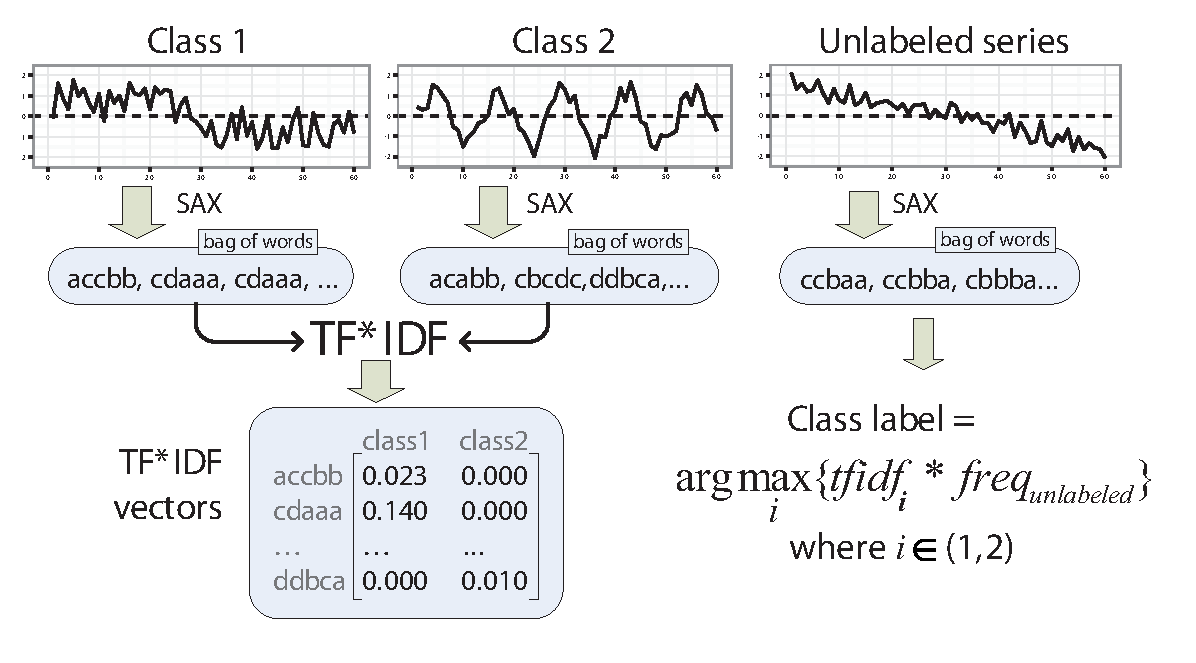
\includegraphics[width=140mm]{figures/overview.eps}
   \caption{
   An overview of SAX-VSM algorithm: 
   at first, labeled time series are converted into bags of words using SAX; 
   secondly, \textit{tf$\ast$idf} statistics is computed resulting in 
   a single weight vector per training class. For classification, an unlabeled 
   time series is converted into a term frequency vector and assigned a 
   label of a weight vector which yields a maximal cosine similarity value.
   This is \textit{ltc.nnn} weighting schema in SMART notation \cite{citeulike:4469058}.}
   \label{fig:overview}
\end{figure}

\subsection{Training phase}
At first, algorithm transforms all labeled 
time series into symbolic representation. For this, it converts time series into SAX
representation configured by four parameters: the sliding window 
length (\textit{W}), the number of PAA frames per window (\textit{P}), 
the SAX alphabet size (\textit{A}), and by the numerosity reduction strategy (\textit{S}) 
(the choice of  these parameters we shall discuss later).
Each of the subsequences, extracted with overlapping sliding window, 
is normalized to unit standard deviation before being processed with PAA 
\cite{citeulike:3815880}. 
If, however, the standard deviation value falls below a fixed threshold, the 
normalization procedure is not applied in order to avoid a possible over-amplification 
of a background noise.

By applying this conversion procedure to all time series from $N$ training classes, 
algorithm builds a corpus of $N$ bags, to which, in turn, it applies \textit{tf$\ast$idf} 
ranking. These steps result in $N$ real-valued weight vectors of equal length 
representing $N$ training classes. 

As shown, because of the need to scan the whole training set, training of SAX-VSM 
classifier is computationally expensive ($O(nm)$). 
However, there is no need to maintain an index of training series, or to keep any of 
them in the memory at a runtime: the algorithm simply iterates over all training time 
series incrementally building a single bag of SAX words for each of training classes. 
Once built and processed with \textit{tf$\ast$idf}, corpus is also discarded - 
only a resulting set of $N$ real-valued weight vectors is retained for classification. 

\subsection{Classification phase}
In order to classify an unlabeled time-series, SAX-VSM transforms it into the 
terms frequency vector using exactly the same sliding window technique and SAX 
parameters that were used within the training phase. 
Then, it computes cosine similarity values between this terms frequency vector and 
$N$ \textit{tf$\ast$idf} weight vectors representing the training classes. 
The unlabeled time series is assigned to the class whose vector yields the maximal 
cosine similarity value.

\subsection{Sliding window size and SAX parameters selection} \label{section-direct}
At this point of SAX-VSM classification algorithm development, it requires a sliding 
window size and SAX parameters to be specified upfront. 
Currently, in order to select optimal parameters values while knowing only a 
training data set, we use a common cross-validation scheme and DIRECT (DIviding RECTangles) 
algorithm, which was introduced in \cite{citeulike:4210208}.
%However, DIRECT optimization scheme is designed to search for global minima of a real 
%valued function over a bound-constrained domain. In order to overcome this limitation, we 
%employ the rounding of reported solution values to the nearest integer.
DIRECT optimization algorithm is designed to search for global minima of a real valued function 
over a bound constrained domain, thus, we use the rounding of a reported solution values 
to the nearest integer.

DIRECT algorithm iteratively performs two procedures - partitioning the search domain, 
and identifying potentially optimal hyper-rectangles (i.e., having potential to contain good
solutions). 
It begins by scaling the search domain to a n-dimensional unit hypercube which is considered 
as potentially optimal. The error function is then evaluated at the center of this hypercube. Next, 
other points are created at one-third of the distance from the center in all coordinate directions. 
The hypercube is then divided into smaller rectangles that are identified by their center point 
and their error function value. This procedure continues interactively until error function
converges.
For brevity, we omit the detailed explanation of the algorithm, and refer the 
interested reader to \cite{citeulike:12563460} for additional details. Figure  \ref{fig:direct-sampling} 
illustrates the application of DIRECT to \textit{SyntheticControl} data set problem.

\begin{figure}[t]
   \centering
   \includegraphics[width=140mm]{figures/figure_direct.eps}
   \caption{Parameters optimization with DIRECT for \textit{SyntheticControl} data set (6 classes). 
   Left panel shows all points sampled by DIRECT in the space $PAA*Window*Alphabet$ where
   red points correspond to high error values in cross-validation experiments, 
   while green points indicate low error values. 
   Note the green points concentration at $W$=42. 
   Middle panel shows an error-rate heat map when the sliding window size is fixed to 42; 
   this figure was obtained by a complete scan of all 432 points of the slice. 
   Right panel shows the optimized by DIRECT sampling. The optimal solution 
   ($W$=42,$P$=8,$A$=4) was found by sampling of 43 points.}
   \label{fig:direct-sampling}
\end{figure}

\subsection{Intuition behind SAX-VSM}
First of all, by combining \textit{\textbf{all}} SAX words extracted from 
\textit{\textbf{all}} time series of single class into a \textit{\textbf{single bag}} of 
words, SAX-VSM manages not only to capture observed intraclass variability, 
but to efficiently ``generalize'' it through smoothing with PAA and SAX.  

Secondly, by partially discarding the original ordering of time series subsequences and
through subsequence normalization, SAX-VSM is capable to capture, and to recognize 
characteristic subsequences in distorted by rotation or shift time series, as well,
as to recover a signal from partially corrupted or altered by noise. 

Thirdly, the \textit{tf$\ast$idf} statistics naturally ``highlights'' terms unique to a
class by assigning them higher weights, while terms observed in multiple classes are 
assigned weights inversely proportional to their interclass presence frequency. 
This weighting scheme improves the selectivity of classification by  lowering a 
contribution of ``confusive'' multi-class terms while increasing a contribution 
of  class' ``defining'' terms to a final similarity value.   

When combined, these features make SAX-VSM time series classification approach 
unique. 
%Ultimately, it compares a set of short overlapping subsequences extracted from a 
%full length of an unlabeled time series with a weighted set of all characteristic subsequences
%representing a training class.
%Thus, an unlabeled time series is classified by its similarity not to a fixed number 
%of sequences (as in kNN classifiers), or to a fixed number of characteristic features 
%(as in shapelets-based classifiers), but by a product of its subsequences similarity to all 
%known subsequences.
Ultimately, algorithm compares a set of subsequences extracted from an unlabeled time series 
with a weighted set of all characteristic subsequences representing a whole of a training class. 
Thus, unknown time series is classified by its similarity not to a given number of ``neighbors'' 
(as in kNN or BOP classifiers), or to a pre-fixed number of characteristic features (as in
shapelets-based classifiers), but by its combined similarity to all known discriminative
subsequences found in a whole class during training.

This, as we shall show, contributes to the excellent classification performance on temporal 
data sets where time series have a very low intraclass similarity at the full length, but 
embed characteristic to the class subsequences. 
%In particular, note SAX-VSM performance 
%on human-driven, aperiodical telemetry stream with a signal loss - ElectricDevices data set
%\cite{bagnal} (Table \ref{perf_table}), as well as our previous experimental results on 
%software process artifact trails \cite{android}.

\section{Results} \label{results}
We have proposed a novel algorithm for time series classification based on SAX
approximation of time series and Vector Space Model called SAX-VSM. Here, we present 
a range of experiments assessing its performance in classification and clustering and show
its ability to provide insight into classification results.

\subsection{Analysis of the classification accuracy}
To evaluate our approach, we selected thirty three data sets. Majority of the data sets was taken 
from the UCR time series repository \cite{citeulike:12563599}, the Ford data set was downloaded from 
IEEE World Congress on Computational Intelligence website \cite{citeulike:12563754}, the 
ElectricDevices data set was downloaded from supporting website for \cite{citeulike:11345338}. 
Overall, SAX-VSM classification performance was found to be at the level of 
1NN classifiers based on Euclidean distance, DTW, or BOP, and a shapelet-tree. 
This result is not surprising taking in account ``No Free Lunch theorems'' \cite{citeulike:404286}, 
which assert, that there will not be a single dominant classifier for all TSC problems.

Table \ref{perf_table} compares the performance of SAX-VSM and four competing 
classifiers: two state-of-the-art 1NN classifiers based on Euclidean distance and DTW, 
the classifier based on the recently proposed Fast-Shapelets technique \cite{citeulike:12563493},
and the classifier based on BOP \cite{citeulike:10525778}. 
We selected these particular techniques in order to position SAX-VSM 
in terms of accuracy and interpretability. 
The presented comparison data sets selection is limited to the number 
of previously published or provided by the authors benchmark results for all of 
four competing classifiers. 
The performance of SAX-VSM for the rest of the data sets \cite{citeulike:12563560}.

In our evaluation, we followed train/test split of the data (exactly as provided by UCR or other
sources). We exclusively used train data in cross-validation experiments for selection of SAX
parameters and numerosity reduction strategy using our DIRECT implementation. 
Once selected, the optimal set of parameters was used to assess SAX-VSM classification 
accuracy which is reported in the last column of the Table \ref{perf_table}.

%\enlargethispage{0.5cm} 
\begin{footnotesize}
\begin{table}[t]
\caption{\bf Classifiers error rates comparison.}
 \label{perf_table}
\centering
\begin{tabularx}{\linewidth}{@{} l *6X @{}}\toprule[1pt]
%\bf Data set &\bf 1NN-Euclidean &\bf 1NN-DTW &\bf Shapelet Tree &\bf  Shapelet SVM &\bf 
%SAX-VSM\\\midrule
%SyntheticControl  & 0.120   & \textbf{0.007}  & 0.057     & 0.127            & 0.010 \\
%Adiac             & 0.389   & 0.396           & 0.700        & 0.762         & \textbf{0.381}\\
%Beef              & 0.467   & 0.467           & 0.500        & 0.133         & \textbf{0.033}\\
%ChlorineConcentration  & 0.350 & 0.350        & 0.412        & 0.439         & \textbf{0.332} \\
%Coffee            & 0.250   & 0.180           & 0.036     & \textbf{0.0}     & \textbf{0.0} \\
%ECG               & 0.120   & 0.230           & 0.149     & \textbf{0.007}   & 0.09 \\
%ElectricDevices   & 0.913   & 0.913           & 0.451     & 0.758            & \textbf{0.329} \\
%FaceFour          & 0.216   & 0.170           & 0.159     & 0.023            & \textbf{0.0} \\
%Gun Point         & 0.087   & 0.093           & 0.107     & \textbf{0.0}     & 0.007 \\
%Lightning7        & 0.425   & \textbf{0.274}  & 0.507     & 0.301            & 0.301 \\
%SonyAIBO          & 0.306   & 0.274           & 0.155     & \textbf{0.133}   & 0.176 \\
%Trace             & 0.240   & \textbf{0.0}    & 0.020     & 0.020            & \textbf{0.0} \\

%\bf Data set &\bf \#Classes &\bf 1NN-Euclidean &\bf 1NN-DTW &\bf Shapelet Tree &\bf  BOP &\bf 
%SAX-VSM\\\midrule
Data set & Nb. of classes & 1NN-Euclidean & 1NN-DTW & Fast Shapelet Tree &  Bag Of \mbox{Patterns}
& SAX-VSM\\\midrule
%50words           &50  & 0.369   & 0.310           &
Adiac             &37  & 0.389   & 0.396           & 0.515        & 0.432         & \textbf{0.381}\\
Beef              &5   & 0.467   & 0.467           & 0.447        & 0.400         & \textbf{0.033}\\
%ChlorineConcentration  & 0.350 & 0.350        & 0.412        & n/a     & \textbf{0.332} \\
CBF             & 3   & 0.148    & 0.003     & 0.053    & 0.013 & \textbf{0.002} \\
Coffee           &2    & 0.250   & 0.180           & 0.067     & 0.036     & \textbf{0.0} \\
ECG200          &2   & \textbf{ 0.120 }  & 0.230           & 0.227     & 0.140   & 0.140 \\
%ElectricDevices   & 0.913   & 0.913           & 0.451     & n/a            & \textbf{0.329} \\
FaceAll        &14     & 0.286   & \textbf{0.192}  & 0.402     & 0.219   & 0.207\\
FaceFour        &4     & 0.216   & 0.170           & 0.089     & 0.011   & \textbf{0.0} \\
Fish               &7   & 0.217   & 0.167           & 0.197    & 0.074   & \textbf{0.017} \\
Gun-Point      &2      & 0.087   & 0.093           & 0.060     & \textbf{0.002}     & 0.007 \\
Lightning2     &2      & 0.246   & \textbf{0.131}  & 0.295     & 0.164            & 0.196 \\
Lightning7     &7      & 0.425   & \textbf{0.274}  & 0.403     & 0.466            & 0.301 \\
Olive Oil      &4   & 0.133   & 0.133  & 0.213     & 0.133            & 0.100\\
OSU Leaf      &6   & 0.483   & 0.409  & 0.359     & 0.236            & \textbf{0.107} \\
%SonyAIBO          & 0.306   & 0.274           & \textbf{0.155}     & n/a-   & 0.176 \\
Syn.Control  &6   & 0.120   & \textbf{0.007}  & 0.081     & 0.037            & 0.010 \\
Swed.Leaf   &15  & 0.213   & 0.210 & 0.270 & \textbf{0.198} & 0.251 \\
Trace            &4   & 0.240   & \textbf{0.0}    & 0.002     & \textbf{0.0} & \textbf{0.0} \\
Two patterns     &4   & 0.090   & \textbf{0.0}    & 0.113   & 0.129      & 0.004 \\
Wafer            &2    & 0.005   & 0.020     & 0.004  & 0.003 & \textbf{0.0006} \\
Yoga             &2    & 0.170   & \textbf{0.164}  & 0.249 & 0.170 & \textbf{0.164} \\
\bottomrule[1pt]
\end{tabularx}
\end{table}
%\hline
%\end{tabular}
\end{footnotesize}

\subsection{Scalability analysis}
For synthetic data sets, it is possible to create as many instances as one needs for
experimentation.
We used CBF \cite{citeulike:12563781} in order to investigate and compare the performance of SAX-VSM and 1NN
Euclidean classifier on increasingly large data sets.

In one series of experiments, we varied a training size from ten to one thousand, while test data
set size remained fixed to ten thousands instances. 
For small training data sets, SAX-VSM was found to be significantly more accurate than 1NN Euclidean
classifier. However, by the time we had more than 500 time series in our training set, there was no
statistically significant difference in accuracy (Fig. \ref{fig:precision-runtime}, left). 
As per the running time cost, due to the comprehensive training, SAX-VSM was found to be more
expensive than 1NN Euclidean classifier on small training sets, but outperformed 1NN on large
training sets.
However, SAX-VSM allows to perform training offline and load \textit{tf$\ast$idf} weight vectors
when needed. If this option can be utilized, our method performs classification significantly
faster than 1NN Euclidean classifier (Fig. \ref{fig:precision-runtime}, right).

In another series of experiments we investigated the scalability of our algorithm with
unrealistic training set sizes - up to one million of instances of each of CBF classes.
As expected, with the grows of a training set size, the curve for a total number of distinct SAX
words and curves for dictionary sizes of each of CBF classes reflected a significant saturation 
(Fig. \ref{fig:venn}, left). For the largest of training sets - one million instances of each
class - the size of the dictionary peaked at 67'324 of distinct words (which is less than 10\% of
all possible words of length 7 from an alphabet of 7 letters), and the longest tf$\ast$idf vector 
accounted for 23'569 values (Fig. \ref{fig:venn}, right). In our opinion, this result reflects two
specificities: the first is that the diversity of words which are possible to encounter in 
CBF dataset is quite limited by its classes configuration and by our choice of SAX 
parameters (smoothing). 
The second specificity is that IDF (Inverse Document Frequency, Equation \ref{formula:idf})
efficiently limits the growth of dictionaries by eliminating those words, which are observed in all
of them.

\begin{figure}[t]
   \centering
   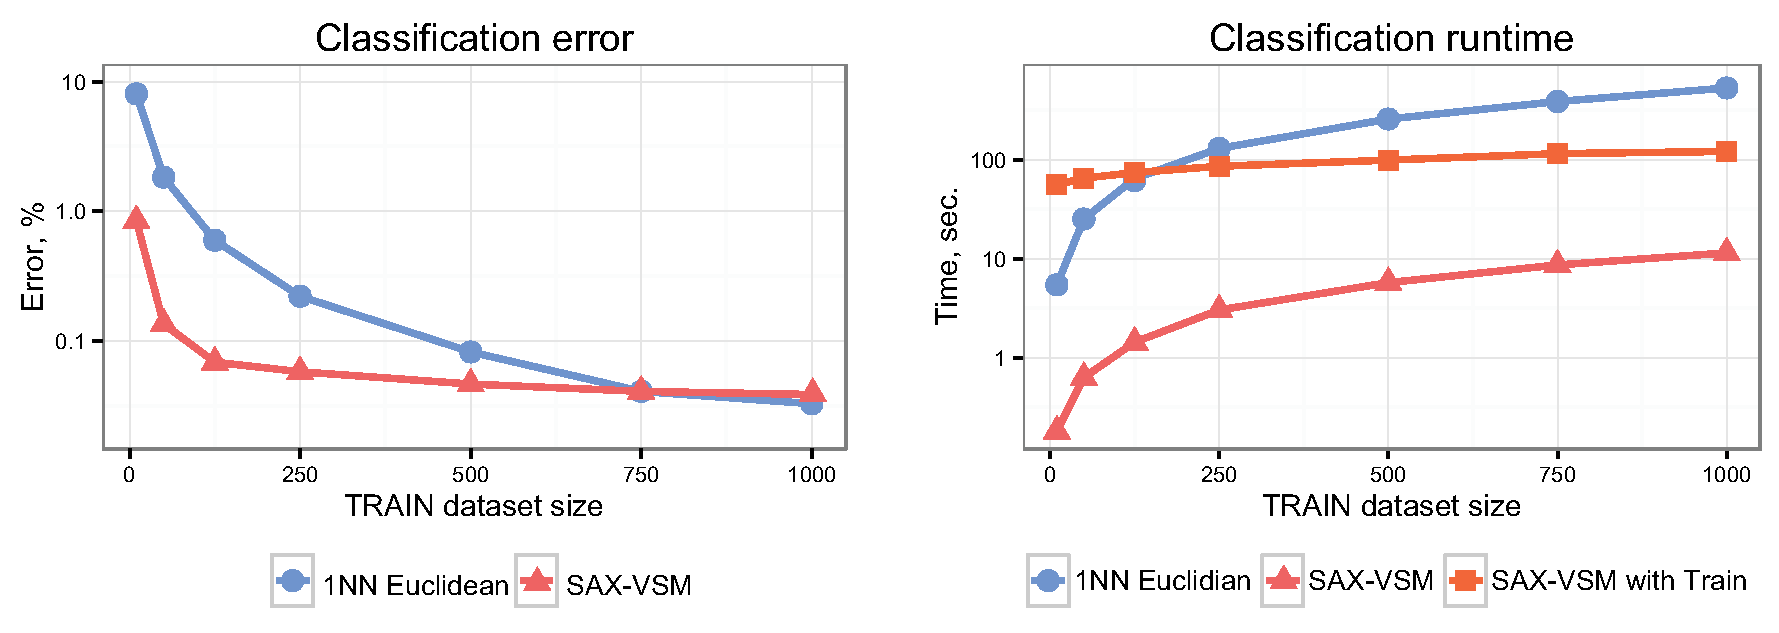
\includegraphics[width=140mm]{figures/precision-runtime.eps}
   \caption{Comparison of classification precision and run time of SAX-VSM and 1NN 
   Euclidean classifier on CBF data. SAX-VSM performs significantly better with limited 
   amount of training samples (left panel). While SAX-VSM is faster in time series 
   classification, its performance is comparable to 1NN Euclidean classifier when 
   training time is accounted for (right panel).}
   \label{fig:precision-runtime}
\end{figure}

%dictionary of the
%with While it grows rapidly at the beginning, once
%the dictionary is saturated, growth tend to slow down (left panel of Figure \ref{fig:corrupted}). 
%Nevertheless, by adjusting alphabet and PAA sizes it is possible to keep the number of terms
%significantly large. 
\begin{figure}[b]
   \centering
   \includegraphics[width=140mm]{figures/Bubbles.eps}
   \caption{Left panel: illustration of dictionaries size evolution for CBF with
   increasingly large training set size. 
   Right panel: distribution of SAX terms in CBF corpus for training set of 
   one million series of each class.}
   \label{fig:venn}
\end{figure}

\subsection{Robustness to noise}
In our experimentation with many data sets, we observed, that the growth of a 
dimensionality of \textit{tf$\ast$idf} weight vectors continuously follows the growth of a
training set size, which indicates that SAX-VSM is actively learning from class variability.
This observation, and the fact that a weight of each of the overlapping SAX words is 
contributing only a small fraction to a final similarity value, prompted an idea that 
SAX-VSM classifier might be robust to the noise and to the partial loss of a signal in
test time series. Intuitively, in such a case, the cosine similarity between high dimensional 
weight vectors might not degrade significantly enough to cause a misclassification.

\begin{figure}[t]
  \centering
  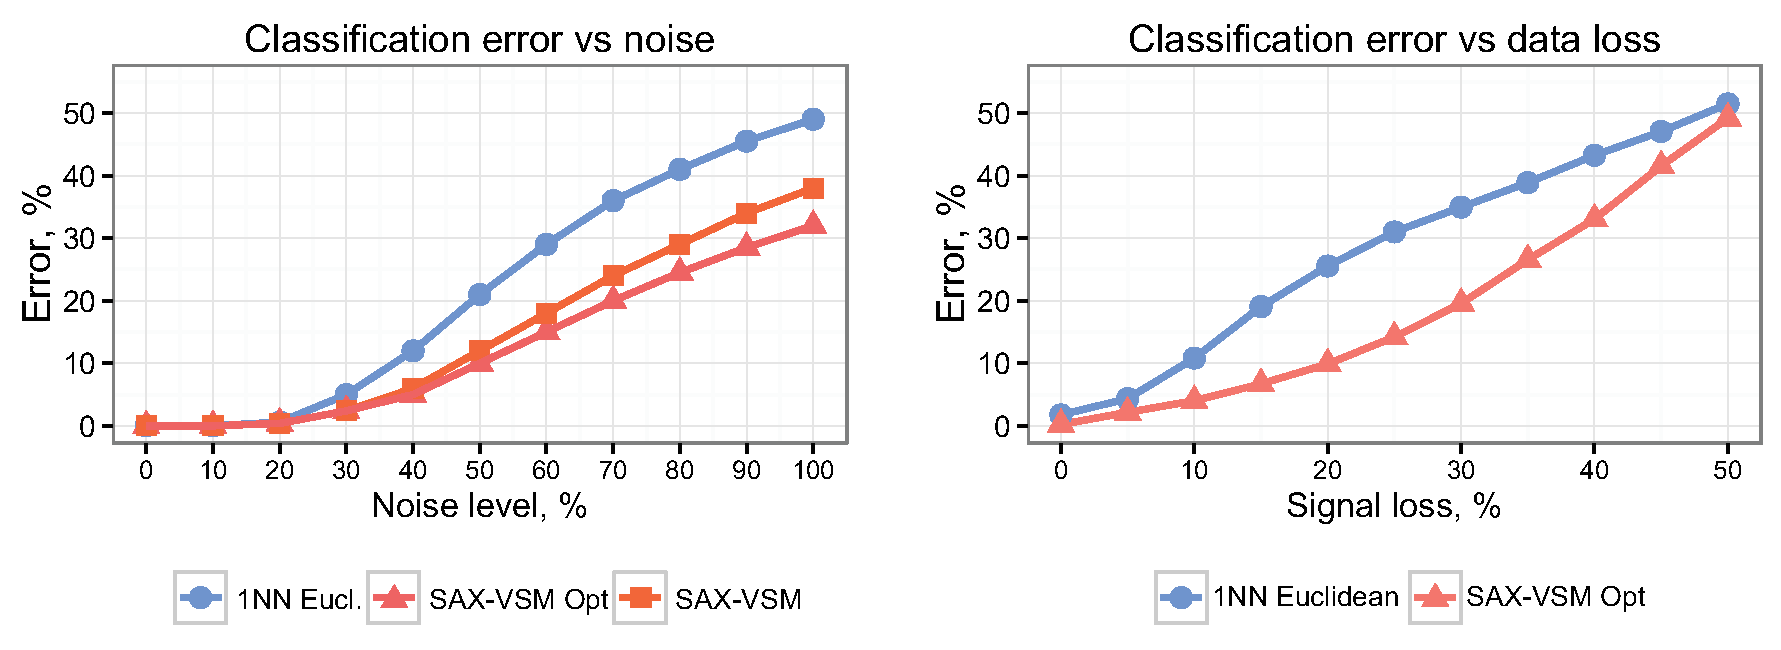
\includegraphics[width=140mm]{figures/corrupted.eps}
  \caption{Classification performance with added noise
  (left panel; the random noise level varies up to 100\% of the signal value,
  and with a signal loss (right panel). \textit{SAX-VSM Opt} curves correspond to 
  results obtained with ``optimized'' for each case SAX parameters 
  (we re-trained a classifier).}
  \label{fig:corrupted}
\end{figure}

While we plan to perform more exploration, current experimentation with CBF data set revealed 
promising results. 
In one series of experiments, by fixing a training set size to two hundred fifty time series, we
varied the standard deviation of Gaussian noise in CBF model (whose default value is about 
17\% of a signal level). We found, that SAX-VSM increasingly outperformed 1NN Euclidean classifier 
with the growth of a noise level (Fig.\ref{fig:corrupted} Left). 
Further improvement of SAX-VSM performance was achieved by fine tuning of smoothing - 
through a gradual increase of the size of SAX sliding window proportionally to the growth of 
a noise level (Fig.\ref{fig:corrupted} Left, \textit{SAX-VSM Opt} curve). 

In another series of experiments, we randomly replaced up to fifty percent of a span of an 
unlabeled time series with a random noise. 
Again, SAX-VSM performed consistently better than 1NN Euclidean classifier regardless of a 
training set size, which we varied from five to one thousand. 
The \textit{SAX-VSM Opt} curve at Fig.\ref{fig:corrupted} (Right) depicts the case
with fifty training series when the sliding window size was decreased inversely proportionally 
to the growth of a signal loss.

\subsection{Interpretable classification}
While the classification performance results in previous sections show that SAX-VSM 
classifier has a very good potential, its major strength is in the level of allowed 
interpretability of classification results. 
%Which, in fact, was our main motivation for this 
%work - to design a classification technique that is not only accurate and reliable, but 
%also highly interpretable, thus can be applicable to the problem of discovery of 
%unknown behaviors \cite{android}.

Previously, in original shapelets work \cite{citeulike:7344347, citeulike:11957982}, it was shown that the 
resulting decision trees provide interpretable classification and offer an insight into the data
specific features. In successive work based on shapelets \cite{citeulike:11345338}, it was shown that
the discovery of multiple shapelets provides even better resolution and intuition into 
the interpretability of classification. 
However, as the authors noted, a time cost of multiple shapelets discovery
in many class problems could be very significant. 
Contrary, SAX-VSM extracts and weights all patterns at once, without any added cost. Thus, it could
be the only choice for interpretable classification in many class problems.

\subsubsection{Heatmap-like visualization}
Since SAX-VSM builds tf$\ast$idf weight vectors using all subsequences extracted from a
training set, it is possible to find out the weight of any arbitrary selected subsequence.
This feature enables a novel visualization technique that can be used to gain an immediate
insight into the layout of ``important'' class-characterizing subsequences as shown at Figure
\ref{fig:heat}.

\begin{figure}[t]
   \centering
   \includegraphics[width=140mm]{figures/CBF-HEAT.eps}
   \caption{An example of the heatmap-like visualization of subsequence ``importance''
   to a class identification. 
   Here, for three CBF time series from a training set, a color value 
   of each point was obtained by combining tf$\ast$idf weights of all patterns 
   which cover the point.
   If a pattern was found in a SAX-VSM-built dictionary corresponding to the 
   time-series class, we added its weight, if, however, a pattern was found in 
   another dictionary - we subtracted its weight. Highlighted by the visualization 
   features corresponding to a sudden rise, plateau, and a sudden drop in Cylinder;
   increasing trend in Bell;
   and to a sudden rise followed by a gradual drop in Funnel, align exactly with the
   design of these classes \cite{citeulike:12563781}.}
   \label{fig:heat}
\end{figure}

\begin{figure}[b]
   \centering
   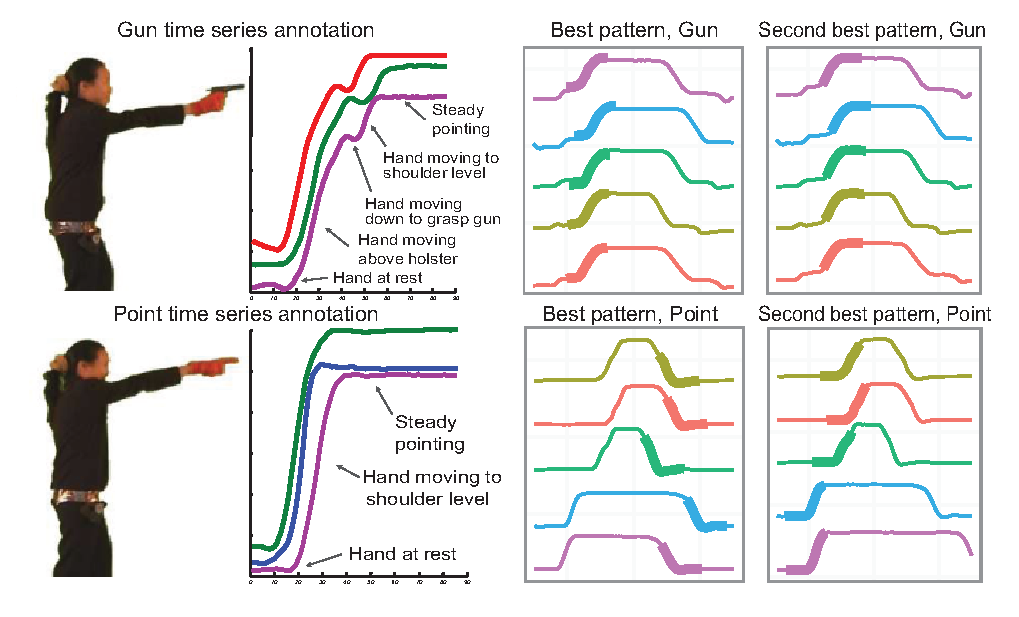
\includegraphics[width=140mm]{figures/gun-point.eps}
   \caption{Best characteristic subsequences (right panels, bold lines) discovered by SAX-VSM in
   \textit{Gun/Point} data set. 
   Left panel shows actor's stills and time series annotations made by an expert, 
   right panels show locations of characteristic subsequences.
   Note, that while the upward arm motion found to be more ``important'' in \textit{Gun} 
   class (gun retrieval and aiming), the downward arm motion better characterizes 
   \textit{Point} class (an ``overshoot'' phenomena in propless arm return). 
   This result aligns with previous work \cite{citeulike:7344347} and \cite{citeulike:11345338}.
   (Stills and annotation used with a permission from E. Keogh) }
   \label{fig:shapelet-like-patterns}
\end{figure}

\subsubsection{Gun Point data set}
Following previously mentioned shapelet-based work \cite{citeulike:7344347, citeulike:11345338}, 
we used a well-studied \textit{GunPoint} data set \cite{DBLP:conf/sdm/RatanamahatanaK04} to explore the 
interpretability of classification results. This data set contains two classes: 
time-series in \textit{Gun} class correspond to the actors' hands motion when drawing
a replicate gun from a hip-mounted holster, pointing it at a target for a second,
and returning the gun to the holster; 
time-series in \textit{Point} class correspond to the actors hands motion when pretending
of drawing a gun - the actors point their index fingers to a target for about a second, 
and then return their hands to their sides. 

Similarly to previously reported results \cite{citeulike:7344347, citeulike:11345338}, 
SAX-VSM was able to capture all distinguishing features as shown at the 
Figure \ref{fig:shapelet-like-patterns}. The most weighted by SAX-VSM patterns in 
\textit{Gun} class corresponds to fine extra movements required to lift and aim the prop. 
The most weighted SAX pattern in \textit{Point} class corresponds to the ``overshoot''
phenomena which is causing the dip in the time series. 
Also, similarly to the original work \cite{DBLP:conf/sdm/RatanamahatanaK04}, SAX-VSM highlighted as second to the best
patterns in \textit{Point} class the lack of distinguishing subtle extra movements required
for lifting a hand above a holster and reaching down for the gun.

\subsubsection{OSU Leaf data set}
According to the original data source, Ashid Grandhi \cite{citeulike:12563798}, with the current growth of
digitized data, there is a huge demand for automatic management and retrieval of various images. The
\textit{OSULeaf} data set consist of curves obtained by color image segmentation and boundary
extraction (in the anti-clockwise direction) from digitized leaf images of six classes: \textit{Acer
Circinatum, Acer Glabrum, Acer Macrophyllum, Acer Negundo, Quercus Garryana and Quercus Kelloggii}.
The authors were able to solve the problem of leaf boundary curves classification by use of DTW, 
achieving 61\% of classification accuracy. However, as we pointed above, DTW provided a
very little information about why it succeeded of failed. 

In contrast, SAX-VSM application yielded a set of class-specific characteristic patterns for each of
six leaves classes from \textit{OSULeaf} data set. These characteristic patterns closely match
known techniques of leaves classification based on leaf shape and margin \cite{citeulike:12134192}. 
Highlighted by SAX-CSM features include the slightly lobed shape and acute tips of
Acer Circinatum leaves, serrated blade of Acer Glabrum leaves, the acuminate tip and characteristic
serration of in Acer Macrophyllum leaves, pinnately compound leaves arrangement of Acer Negundo, the
incised leaf margin of Quercus Kelloggii, and a lobed leaf structure of Quercus Garryana. 
Figure \ref{fig:shapelet-acer-patterns} shows a subset of these characteristic patterns and original
leaf images with highlighted corresponding features.

\begin{figure}[t]
   \centering
   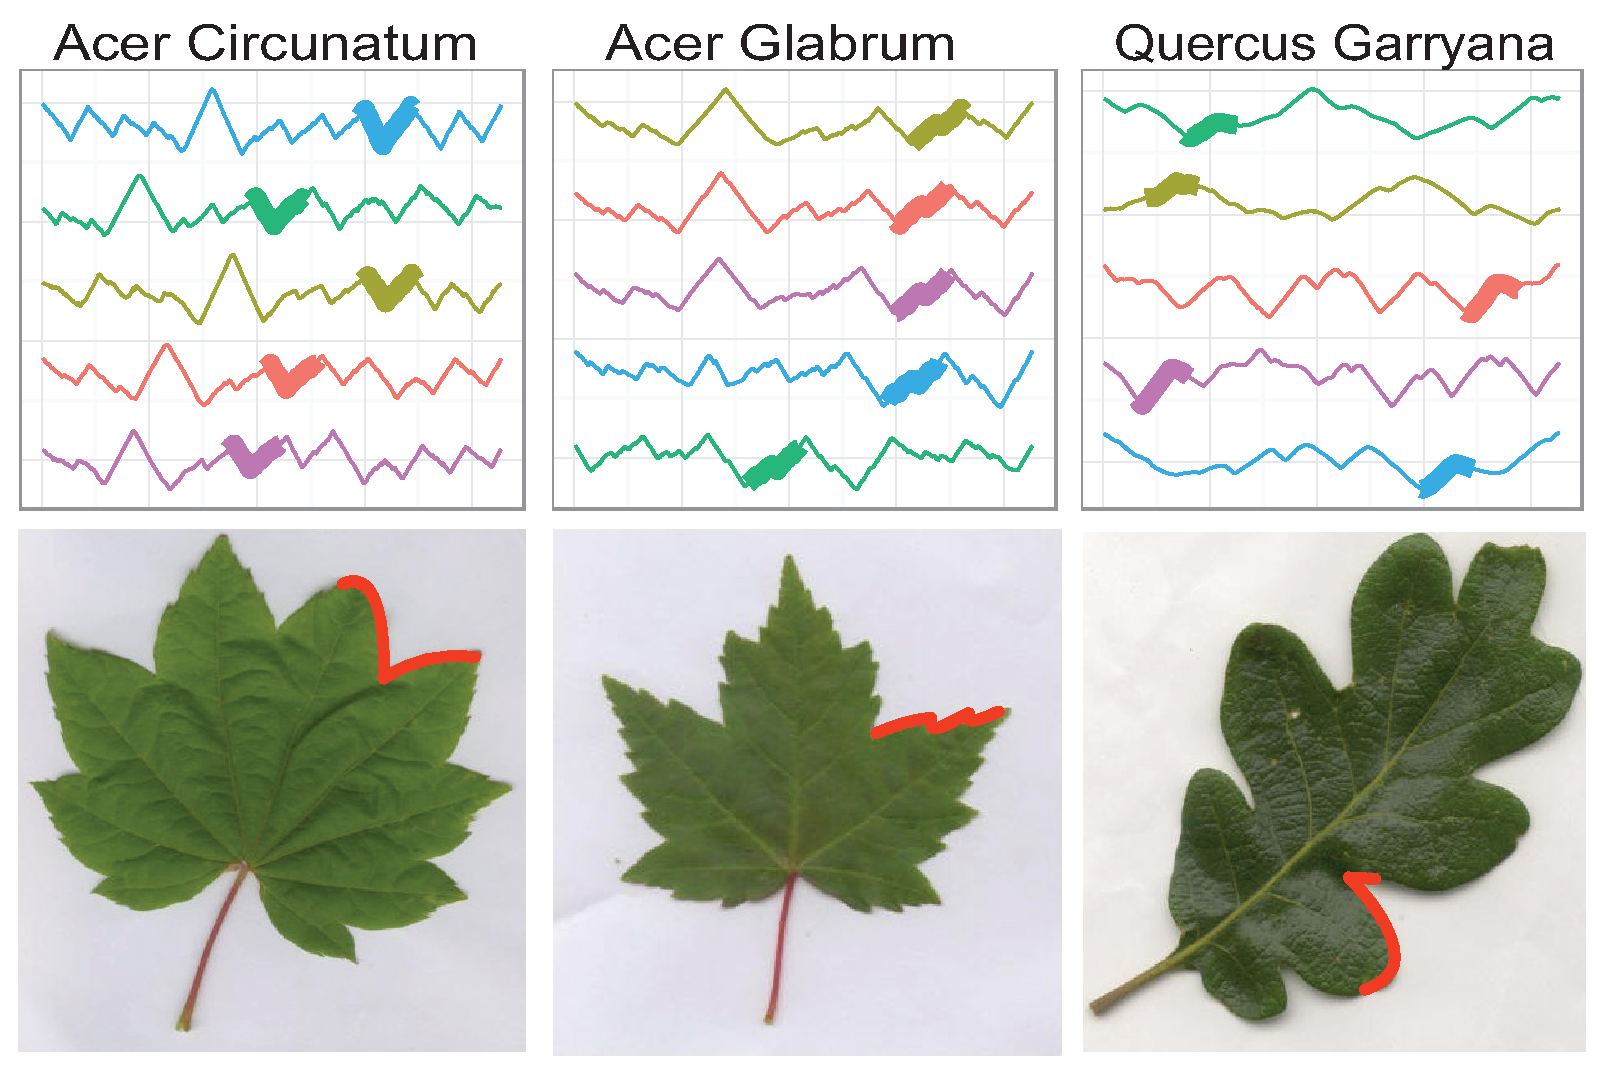
\includegraphics[width=140mm]{figures/AcerCircunatum.eps}
   \caption{Best characteristic subsequences (top panels, bold lines) discovered by SAX-VSM in
      \textit{OSULeaf data set}.
These patterns align with well known in botany discrimination techniques
by lobe shapes, serrations, and leaf tip types \cite{citeulike:12134192}.}
   \label{fig:shapelet-acer-patterns}
\end{figure}

\begin{figure}[t]
   \centering
   \includegraphics[width=140mm]{figures/coffee_patterns.ps}
   \caption{
   Best characteristic subsequences (left panels, bold lines) discovered by SAX-VSM in
   {Coffee data set}. Right panels show zoom-in view on these subsequences in Arabica
   and Robusta spectrograms.
   These discriminative subsequences correspond to chlorogenic acid (best subsequence) 
   and to caffeine (second to best) regions of spectra. This result aligns with
   the original work based on PCA \cite{citeulike:12550833} exactly.
   %Best characteristic subsequences discovered by SAX-VSM in \textit{Coffee data set}.
   %The best subsequences in both classes correspond to chlorogenic acid, while
   %second to best subsequences - to caffeine. This result aligns with previous 
   %exploratory research based on PCA \cite{citeulike:12550833}.
   }
   \label{fig:coffee}
\end{figure}

\subsubsection{Coffee data set}
Another illustration of interpretable classification with SAX-VSM is based on the analysis of its
performance on Coffee dataset \cite{citeulike:12550833}. The curves in this dataset correspond to spectra
obtained with diffuse reflection infrared Fourier transform (DRIFT) and truncated to 286 data points
in the region 800-1900 cm$^{-1}$. The two top-ranked by SAX-VSM subsequences in both datasets
correpond to spectrogram intervals of Chlorogenic acid (best) and Caffeine (second to best).
These two chemical compounds are known to be responsible for the flavor differences in 
Arabica and Robusta coffees; moreover, these spectrogram intervals were reported 
as discriminative when used in PCA-based technique by the authors of the original work
\cite{citeulike:12550833}.

\section{Clustering}
Clustering is a common tool used for data partitioning, visualization, exploration, and serves as
an important subroutine in many data mining algorithms. Typically, clustering algorithms
are built upon a distance function, and the overall performance of an algorithm is highly
dependent on a performance of the chosen function. Thus, an experimental evaluation of the 
proposed technique in clustering provides an additional perspective on its performance and
applicability beyond the classification.

\subsection{Hierarchical clustering}
Probably, one of the most used clustering algorithms is hierarchical clustering which requires no
parameters to be specified \cite{citeulike:1576606}. It computes pairwise distances between all objects and 
produces a nested hierarchy of clusters offering a great data visualization power. 

Previously, it was shown that the bag-of-patterns time series representation and Euclidean distance
provide a superior clustering performance\cite{citeulike:10525778}. 
For comparison, we performed similar experiments which differ in time series representation and
distance metric - we relied on \textit{tf$\ast$idf} weight vectors and cosine similarity. 
Affirming the previous work, we found, that the combination of SAX and Vector space model
outperforms classical shape-based distance metrics. 
For example, figure \ref{fig:hc} depicts the result of hierarchical clustering of a subset of
\textit{SyntheticControl} data. 
As one can see, SAX-VSM is superior in clustering performance to Euclidean and DTW distance 
metrics in this particular setup - it produced a hierarchy which properly partitions the
data set into three branches.

\subsection{k-Means clustering}
Another popular choice for data partitioning is k-Means clustering algorithm \cite{kmeans}.
The basic intuition behind this algorithm is that through the iterative reassignment of objects 
into different clusters the intra-cluster distance is minimized. As was shown, k-Means 
algorithm scales much better than hierarchical partitioning techniques \cite{citeulike:4195343}.
Fortunately, this clustering technique is well studied in IR field. Previously, in \cite{citeulike:505248}, the
authors extensively examined seven different criterion functions for partitional document
clustering and found, that \textit{k}-prototypes partitioning with cosine dissimilarity delivers an
excellent performance. 

Following this work, we implemented a similar to \cite{citeulike:1172599} \textit{spherical k-means algorithm}
and found, that algorithm converges quickly and delivers a satisfactory partitioning on short
synthetic data sets. Further, we evaluated our technique on the long time series from PhysioNet 
archive \cite{citeulike:699487}. 
We extracted two hundred fifty series corresponding to five vital signals: two ECG leads 
(aVR and II), and RESP, PLETH, and CO2 waves, trimming them to 2'048 points. Similarly to
\cite{citeulike:10525778}, we run a reference k-Means algorithm implementation based on Euclidean
distance, which achieved the maximum clustering quality of 0.39, when measured as proposed in
\cite{citeulike:1325189} on the best clustering (the one with the smallest objective function in 10 runs). 
SAX-VSM spherical k-Means implementation outperformed the reference technique yielding 
clusters  with the quality of 0.67 (on 10 runs with SAX parameters set to 
$W$=33, $P$=8, $A$=6).

%Note also, that previously, we applied our implementation to recurrent behaviors (motifs) 
%discovery in software development telemetry streams\cite{android}. 
%These behavioral time series were extracted from software change repositories and are 
%structurally similar to \textit{ElectricDevices} data set. 
%We used our \textit{tf$\ast$idf} weight vectors time series representation and spherical 
%k-Means implementation in order to discover specific temporal features corresponding 
%to the software release cycle. 
%Specifically, we optimized SAX parameters in order to obtain a proper partitioning of known 
%development behaviors before and after the software release. 
%In turn, the centroids of these clusters represented by \textit{tf$\ast$idf} weight vectors 
%were used to classify unlabeled  temporal intervals. 
%This technique allowed us to successfully classify pre- and post-release
%behaviors with accuracy above 80\%.

\begin{figure}[t]
   \centering
   \includegraphics[width=140mm]{figures/clustering.eps}
   \caption{An comparison of hierarchical clustering application to a subset of three
   \textit{SyntheticControl} classes: \textit{Normal, Decreasing trend}, and \textit{Upward shift}. 
   Euclidean distance, Dynamic time warping, SAX-VSM and Complete linkage were used to 
   generate these plots. Only SAX-VSM was able to partition series properly.                       
   }
   \label{fig:hc}
\end{figure}

\section{Conclusion and Future Work} \label{conclusion}
In this paper, we have proposed a novel interpretable technique for time series classification
based on characteristic patterns discovery. We have shown, that our approach is competitive with, 
or superior to, other techniques on a variety of classic data mining problems. In addition, 
we described several advantages of SAX-VSM over existing structure-based similarity measures,
emphasizing its capacity to discover and rank short subsequences by their class characterization
power.

The current limitations of our SAX-VSM implementation suggest a number of future work directions. 
First of all, while Vector space model naturally supports processing of bags of words composed 
of terms of variable length, our current ``stable'' implementation lacks this capacity.
Inspired by the recently reported superior performance of multi-shapelets based classifiers
\cite{citeulike:11345338}, we prioritize this development.
Secondly, as mentioned before, DIRECT optimization it is designed for a function of a real variable.
By using rounding in our implementation, we have observed DIRECT iteratively sampling redundant
locations in suboptimal neighborhood, thus, a more appropriate optimization scheme is needed.
Finally, we are designing and experimenting with an extension of SAX-VSM to multidimensional time
series. Currently we are evaluating two candidate implementations: the first is based on a
single bag of words accommodating all dimensions for a class (by prefixing SAX words extracted from
different dimensions); while the second is based on the use of a single bag of words per each of
dimensions. The preliminary results on synthetic data sets look promising and we expect to report 
our finding soon.
